\section{Methodology}
\label{sec:dataset:architecture:methodology}

To understand the methodology on how we captured our dataset, we must first introduce the three key notions behind \gls{mde}: technical spaces, models and systems. A system is a concrete ``group or set of related or associated elements perceived or thought of as a unity or complex whole'' \citep{oed:system}. Technical spaces were introduced by \citet{Bezivin:2002} as a model management framework based on algebraic structures (e.g., trees, (hyper)graphs, categories). Technical spaces are usually based on a three-tier conjecture: metametamodels, metamodels and models. Whereas a model is an abstract representation of  a concrete system of specific purpose, a \textit{meta}model, in contrast, describes the way to describe those models. A \textit{metameta}model can be used to describe the representation structure of our metamodels and defines a type system \cite{Cardelli:1985ee} that supports all underlying layers \citep{Bezivin:2006gw}. \cref{fig:dataset:bezivin2006_metamodel} captures these concepts in further detail.

\begin{figure}[h]
  \centering
  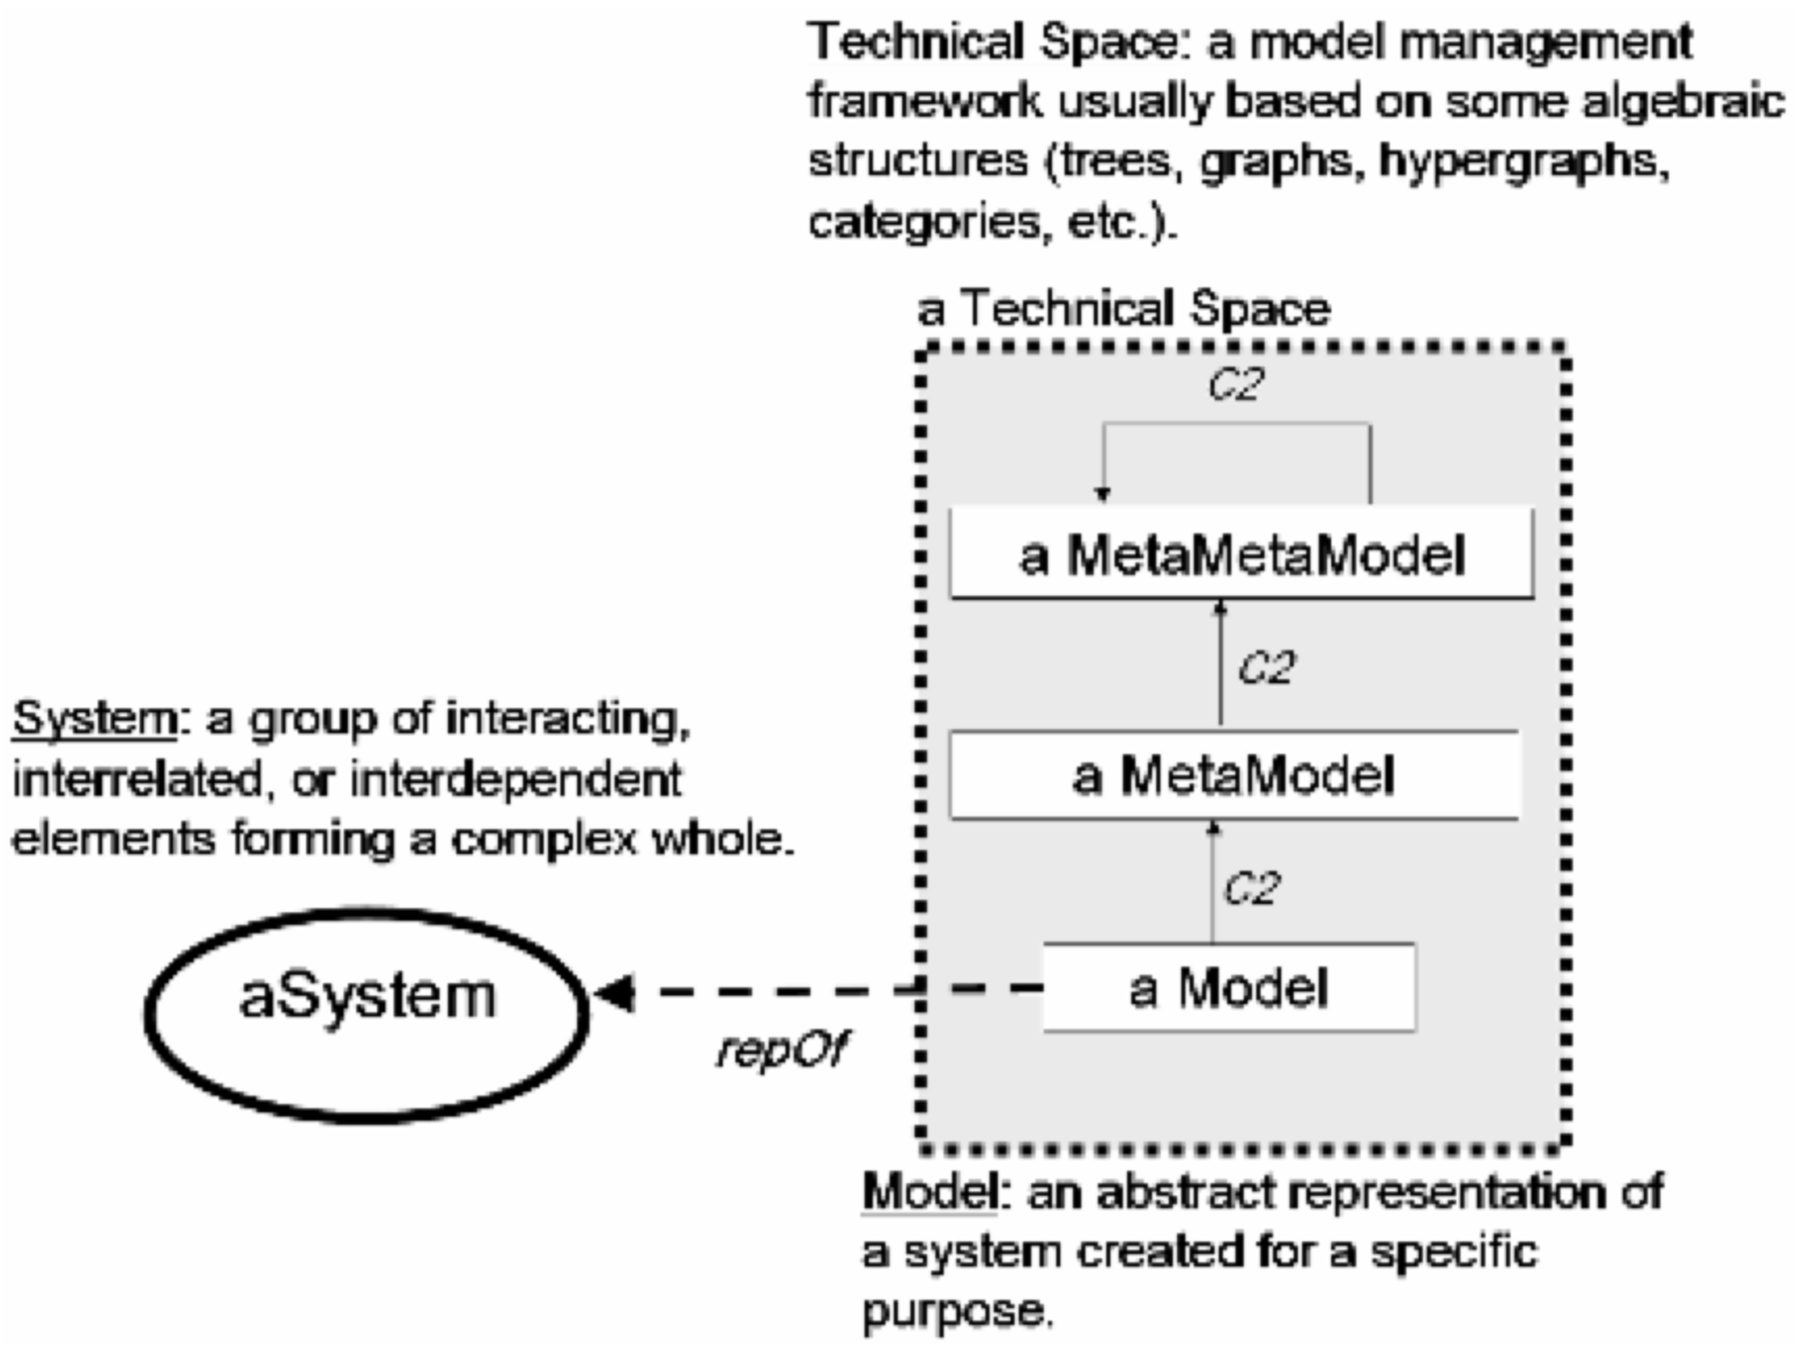
\includegraphics[width=0.6\textwidth]{images/dataset/bezivin2006_metamodel}
  \caption[An overview of systems, models and technical spaces]{Systems, models and technical spaces. (From \citep{Bezivin:2006gw}.)}
  \label{fig:dataset:bezivin2006_metamodel}
\end{figure}

We conceptualise our technical space as a series of layers (\cref{fig:dataset:layers}), whereby the innermost layer is the metamodel and the outermost layer is the system. To develop our metamodel, we adopt a pragmatic approach by working \textit{backwards} from the system to the metamodel: using a prototypical exploration process, we developed a prototype system (\textit{Argus}, described in \cref{ch:argus}) iteratively with a data tagging team who manually curated the data by observing what features were missing. We use the term \textit{iteration} to refer to the process of deploying Argus to the data tagging team, capturing a set of photos from various races, and sending the data back for quality assurance. Once this prototype was stable, we conceptualised a model (\cref{sec:dataset:architecture:what_to_capture}) from the prototype to describe what it is that Argus captures. We then generalised that model, expanding from a model that was marathon-specific, into a more generalisable metamodel (\cref{sec:dataset:architecture:metamodel}). We represent this overall process as as a \gls{uml} activity sequence diagram, shown in \cref{fig:dataset:methodology}.

Formally, we adopt a mixed methods approach that combines a quasi-experimental design with an observational study \citep{Trochim:2001wg,Gray:2013va}: each of these iterations are considered as a quasi-experiment, where the previous iteration acts as a control to the following iteration on without random assignment. Between iterations, we apply a treatment (software improvement) that we deduce from an observational assessment on the behaviour on how people use the software, and therefore to determine how to improve our tagging tool.

\begin{figure}[h]
  \centering
  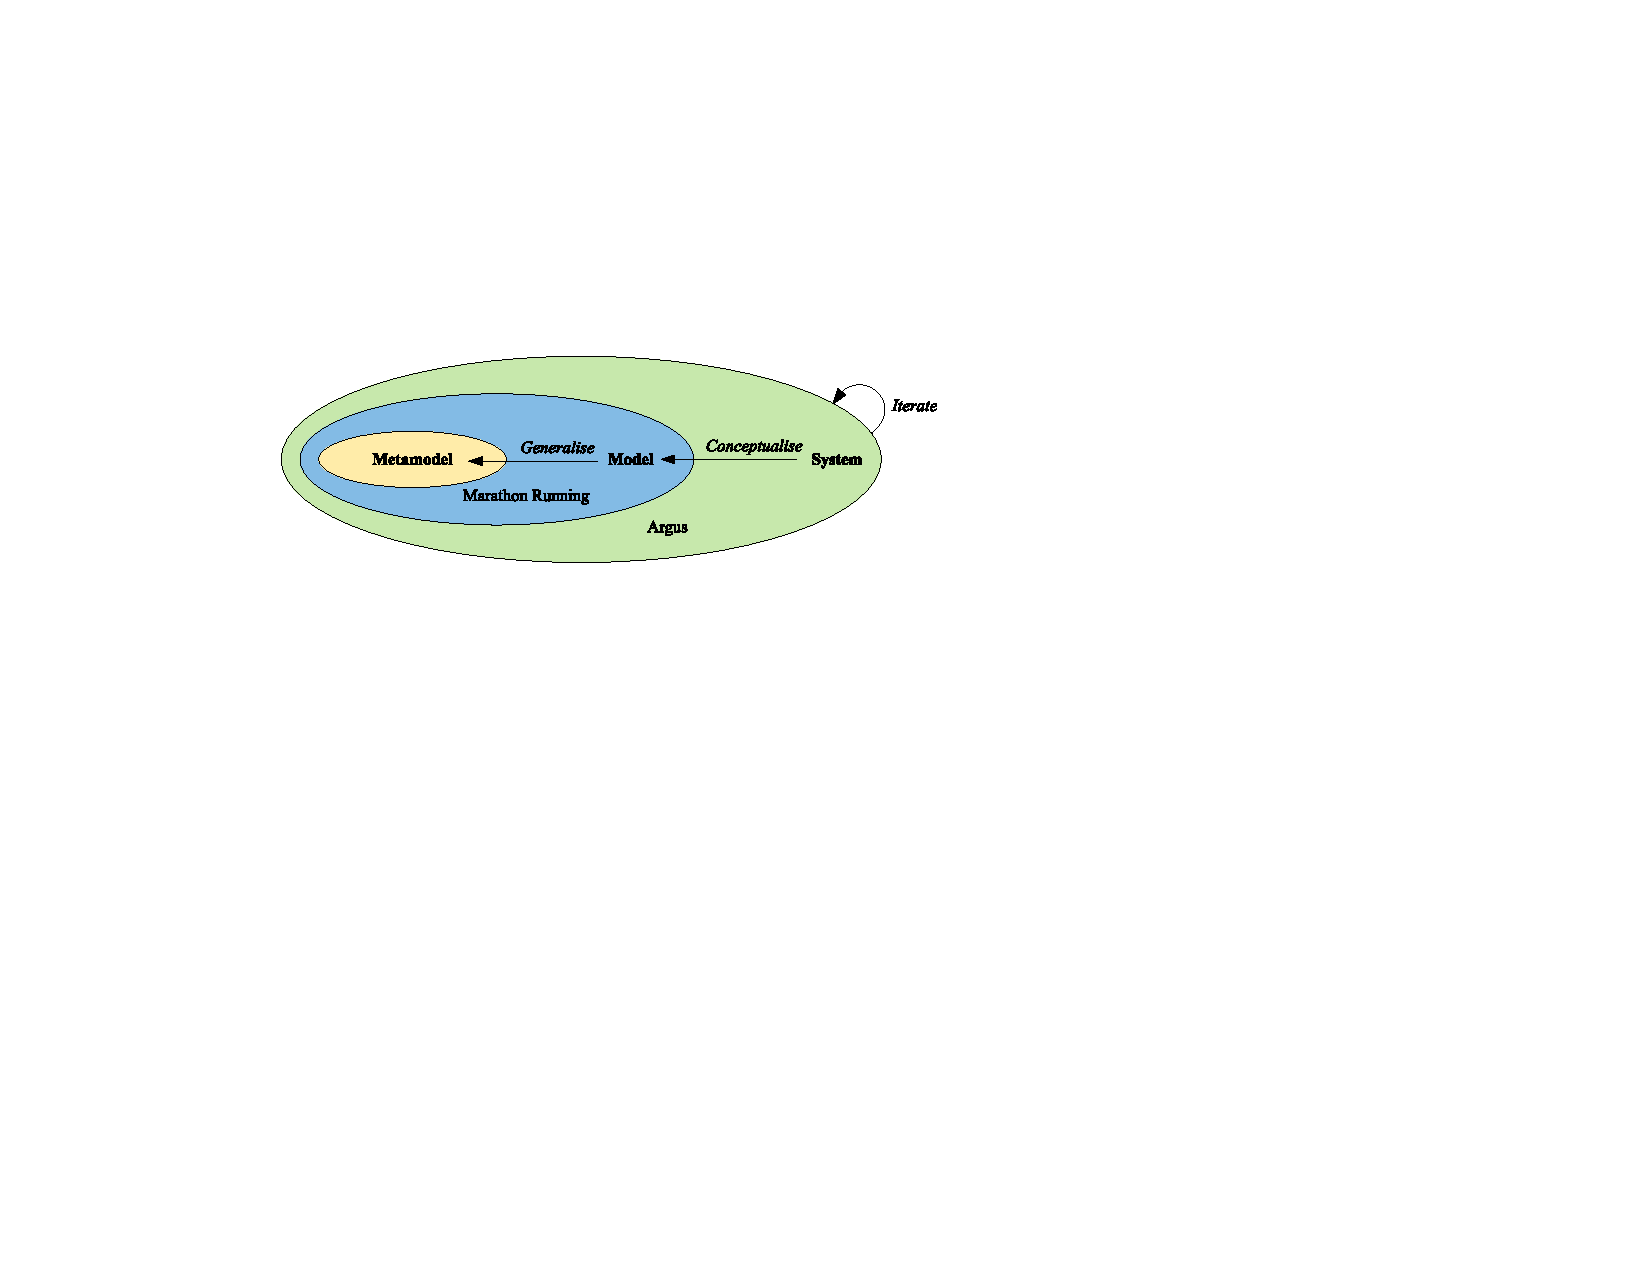
\includegraphics[width=0.8\textwidth]{images/dataset/layers}
  \caption[A layered approach to develop our metamodel]{A layered discovery process from iteratively designing a system, conceptualising the system to a model, and generalising the model into a metamodel.}
  \label{fig:dataset:layers}
\end{figure}

The initial phase in our dataset development was to create a prototype system with the specific purpose of tagging our marathon runner context (using the dataset provided by the industry client).

%We name this partial implementation \textit{Argus}\footnoteurl{http://www.deakin.edu.au/~ca/argus}{5 July 2017}. Refer to \cref{sec:dataset:argus} for more about this implementation. 

To develop a model (that informed our metamodel would), we began by discussing what requirements were needed---that is, the key features that we thought were necessary for extracting from our image. Five features were decided: (1) the crowdedness of the photo, (2) the visible bib sheets within the photo, (3) the faces corresponding to those bib sheets, (4) the prominence of runners of the photo and (5) the colours of runners' clothing in the photo.

Once an initial prototype was developed, we conducted informal usability tests with members from \gls{dstil}\footnote{These members were research colleagues. Refer to \cref{ch:ethics_clearance}.}, which captured minor flaws in the workflow (namely required conditions that were missing in annotations) as well as general usability enhancements. We achieved an average \gls{sus} score \citep{Jordan:1996wa} of 70 of 100. These are noted in \cref{ch:usability}. Once the internal testing had concluded, we developed instructional video guides on how to use Argus, and then deployed the tool to a remote data tagging team.

We ran four iterations of tagging with our remote data tagging team. These iterations consisted of photos from different marathon races in our dataset. (To ensure variance in tagging, there were some races at night and some races with alphanumeric components in the \gls{rbn}.) After each iteration, the research team assessed the tagging for quality. We explain this quality evaluation further in \cref{sec:dataset:argus:quality_eval}. Feedback identified further restrictions that needed to be placed on Argus as poor approximations or incorrect tagging would cause our \gls{ai} to learn poorly. 

The following issues were identified:

\begin{itemize}
  \item face region was too far away from the bib region,
  \item face region was overlapping the bib region,
  \item \glspl{rbn} had spaces,
  \item misidentified \glspl{rbn} where the alphabetic `I' was tagged as the numeric `1'.
\end{itemize}
\noindent
To prevent further training photos from being labelled with incorrect data, and therefore improperly train the \gls{nn},  we added geometric restrictions and conditions into the tool to prevent these errors from occurring at all (i.e., ensuring faces could only be marked above and horizontally near bibs). We also ensured that only alphanumeric characters can be entered as \glspl{rbn}. Some of these issues are highlighted in \cref{fig:dataset:issues_with_tagging}.

\begin{figure}[p]
  \centering
  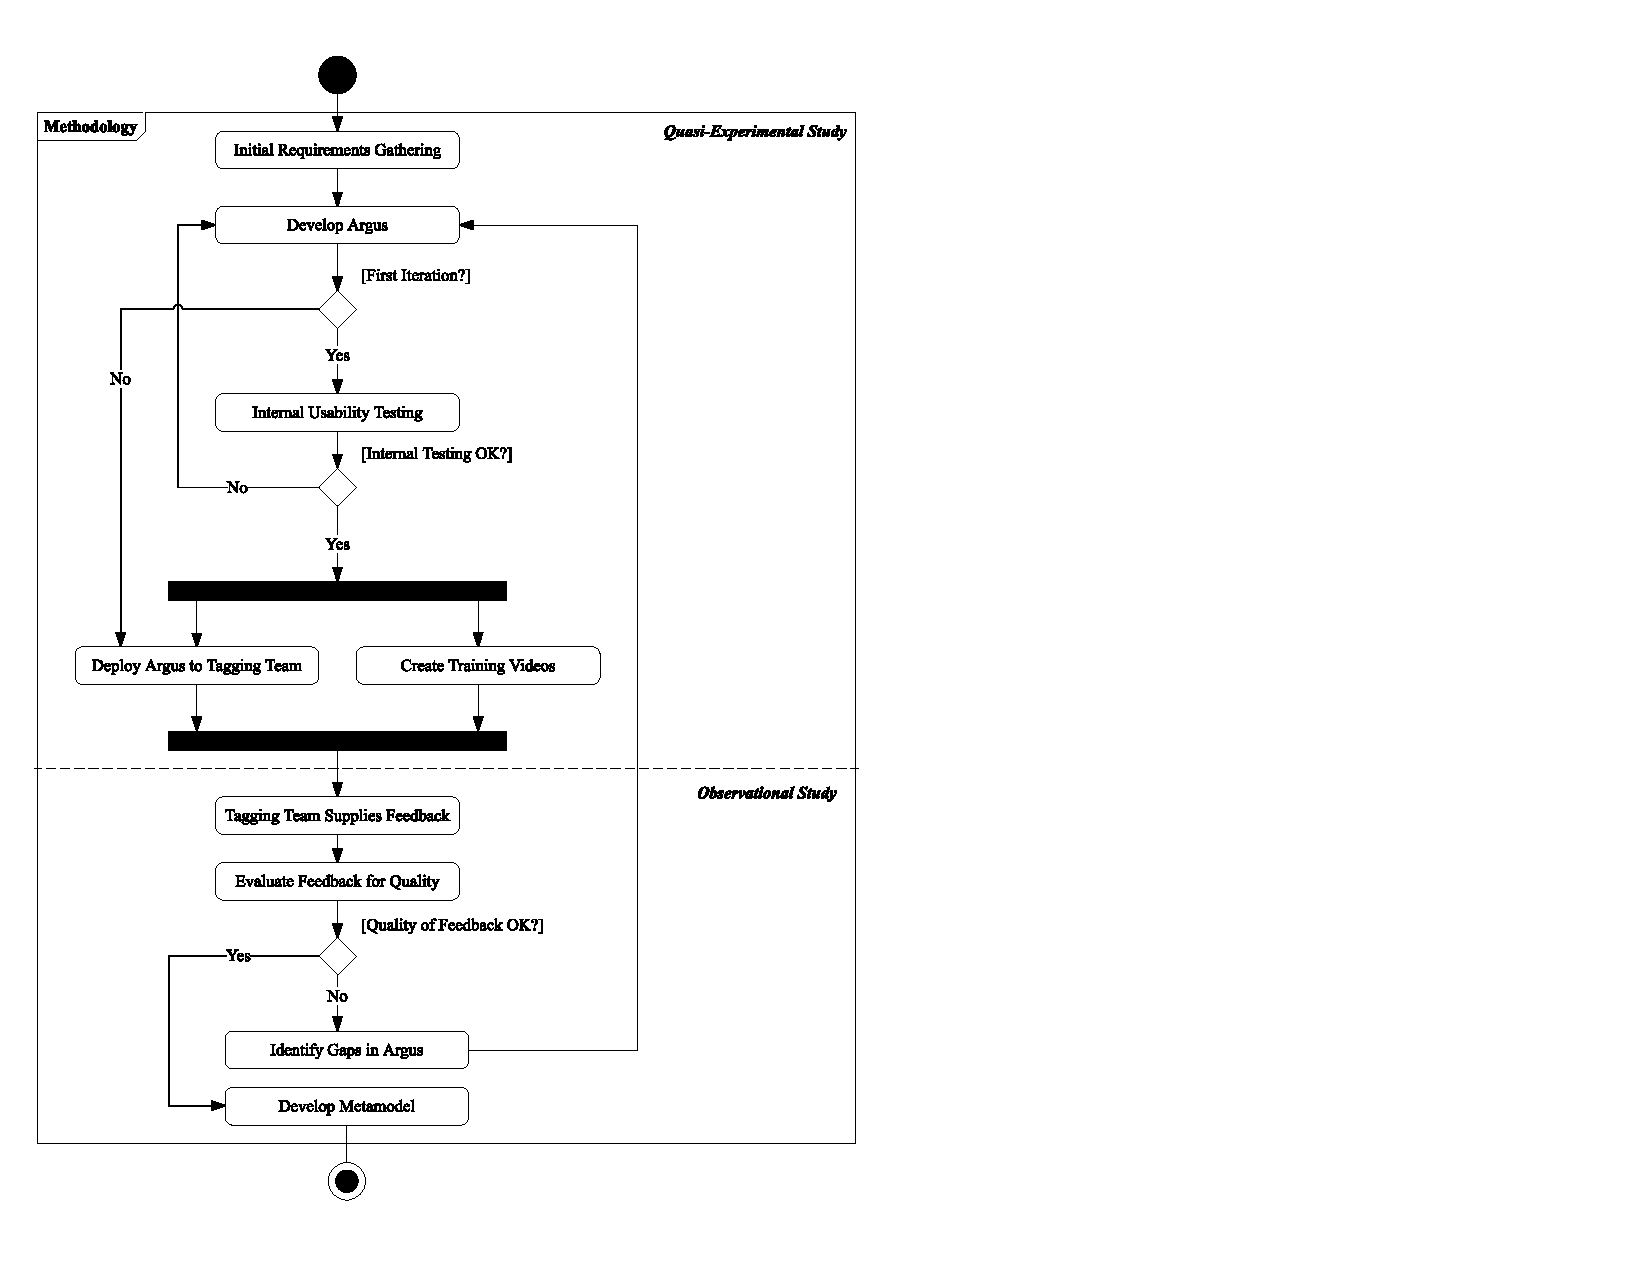
\includegraphics[width=\textwidth]{images/dataset/methodology}
  \caption[Implementation methodology]{An overview of the methodology used to discover our metamodel. Formally, we consider our approach to be a mixed methods approach between a quasi-experimental and observational study for the relevant states.}
  \label{fig:dataset:methodology}
\end{figure}
